\section{Техническое задание}
\subsection{Основание для разработки}

Основанием для разработки является задание на курсовую работу «\Тема».

\subsection{Цель и назначение разработки}

Задачами данной разработки являются:
\begin{itemize}
\item осуществление загрузки аудиофайла и извлеения аудиоданных;
\item реализация отображения аудиоданных посредством аудиодорожки;
\item создание способов обработки аудиоданных;
\item осуществление сохранения изменений и запись аудиофайла.
\end{itemize}

\subsection{Требования пользователя к интерфейсу программы}

Программа должна включать в себя:
\begin{itemize}
    \item возможность выбора аудиофайла;
    \item визуализацию аудиофайла;
    \item набор инструментов для манипуляции аудиофайлом;
    \item возможность сохранения аудиофайла;
\end{itemize}

Композиция программы представлена на рисунке ~\ref{test_image:image}.

\begin{figure}[ht]
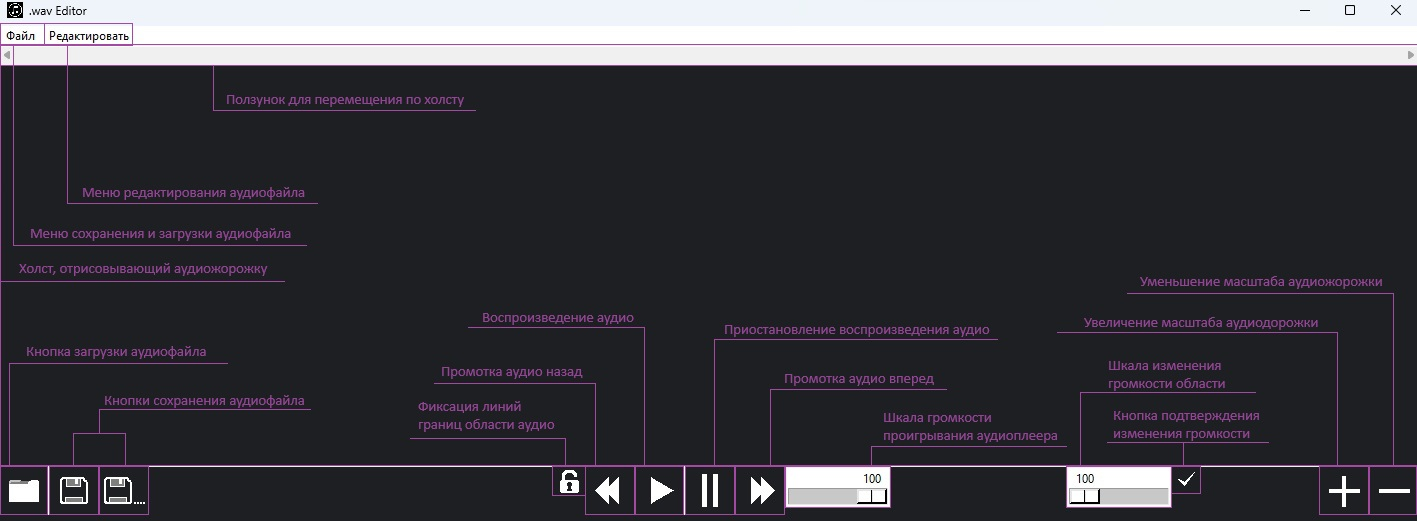
\includegraphics[width=1\linewidth]{test_image}
\caption{Композиция интерфейса программы}
\label{test_image:image}
\end{figure}
%\vspace{-\figureaboveskip} % двойной отступ не нужен (можно использовать, если раздел заканчивается картинкой)

\subsection{Моделирование вариантов использования}

Для разрабатываемой программы была реализована модель, которая обеспечивает наглядное представление вариантов использования аудиоредактора.

Она помогает в физической разработке и детальном анализе взаимосвязей объектов. При построении диаграммы вариантов использования применяется унифицированный язык визуального моделирования UML.

Диаграмма прецедентов (рис. \ref{diagram_choice:image}) описывает функциональное назначение разрабатываемой программы. То есть это то, что программа будет непосредственно делать в процессе своего функционирования. Проектируемая программа представляется в виде ряда прецедентов, предоставляемых системой актерам или сущностям, которые взаимодействуют с ней. Актером или действующим лицом является сущность, взаимодействующая с программой извне. Прецедент служит для описания набора действий, которые программа предоставляет актеру. 

На основании анализа предметной области в программе должны быть реализованы следующие прецеденты работы с аудиофайлом, все прецеденты осуществляются посредством взаимодействия с компонентами интерфейса:
\begin{enumerate}
\item Загрузка - возможность выбора аудиофайла для последующей визализации и редактирования.
\item Визуализация - отображение аудиоданных в виде аудиодорожки с возможностью увеличения и уменьшения масштаба, а также выбора необходимой области.
\item Прослушивание - возможность воспроизведения и остановки прослушивания аудио, также как и перемотки на определенное количество секунд вперед/назад.
\item Редактирование - наличие набора инструментов для редактирования аудиоданных, включающего в себя такие операции, как копирование, удаление, вставку, замену, обнуление, добавление эффекта нарастания и затухания и изменение громкости.
\item Сохранение - возможность записи измененных аудиоданных в WAV файл, как новый, так и оригинальный.
\end{enumerate}

\begin{figure}[ht]
	\includegraphics[width=1\linewidth]{diagram_choice}
	\caption{Диаграмма прецедентов}
	\label{diagram_choice:image}
\end{figure}

\subsection{Нефункциональные требования к программной системе}

\subsubsection{Требования к надежности}
В связи с тем, что работа в программе ведется не с самим файлом непосредственно, а с буфером данных, получаемых из него,
то даже при удалении исходного аудиофайла все данные о нем будут сохранены в случае, если они уже были загружены в программу.

\subsubsection{Требования к программному обеспечению}
Для реализации программы должен быть использован язык Python, а также связанные с ним библиотеки: Tkinter, PySDL, NumPy и Ctypes. Для корректной работы программы должен быть установлен Python версии не ниже 3.11.

\subsubsection{Требования к аппаратному обеспечению}
Для корректной работоспособности программы необходим процессор с 2 и более ядрами.
Объем оперативной памяти должен быть не менее 512 МБ.

\subsection{Требования к оформлению документации}

Разработка программной документации и программного изделия должна производиться согласно ГОСТ 19.102-77 и ГОСТ 34.601-90. Единая система программной документации.
